
\begin{figure}[t]
\begin{tikzpicture}
\node(py)[scale=0.9,inner ysep=0] {
\begin{lstlisting}[language=python]
import numpy as np

def kmeans(X:np.ndarray, k:int, niters:int):
    # initialization
    centroids = X[np.random.choice(X.shape[0], k)]
    clusters = list[list[int]]()
    for i in range(niters):
        # loop body
        clusters = [list[int]() for _ in range(k)]
        for sample_i in range(len(X)):
            v = X[sample_i] - centroids
            r = np.linalg.norm(v, None, 1).argmin()
            clusters[r].append(sample_i)
        new_centroids = np.array([X[cluster].mean(0)
                             for cluster in clusters])
        if np.allclose(centroids, new_centroids):
            break
        centroids = new_centroids
    # finalization
    return compute_labels(clusters, X.shape[0])
\end{lstlisting}
};
\node(pseudo)[right=0 of py.north east,
anchor=north west, scale=0.7] {
\begin{minipage}{9cm}
\begin{algorithmic}
\Function{kmeans}{$X$, $k$, $n$}
\State $\mathit{centroids} \gets \textrm{choose}~
  \{C\subseteq X \mid |C|=k\}$
\Loop ~(max $n$ iterations)
  \State $\mathit{clusters} \gets \big\{
    \{p\in X \mid p \textrm{~is closest to~} c\}$ 
  \State \hspace{3.5cm} $~\big|~ c\in \mathit{centroids} \big\}$
  \State $\mathit{centroids}' \gets \{\mu(C) \mid
    C \in \mathit{clusters}\}$
  \If {$\mathit{centroids}' \approx \mathit{centroids}$}
    \State \textbf{break}
  \Else
    \State $\mathit{centroids} \gets \mathit{centroids}'$
  \EndIf
\EndLoop
\EndFunction
\end{algorithmic}
\end{minipage}
};

\node[below=0 of pseudo] {
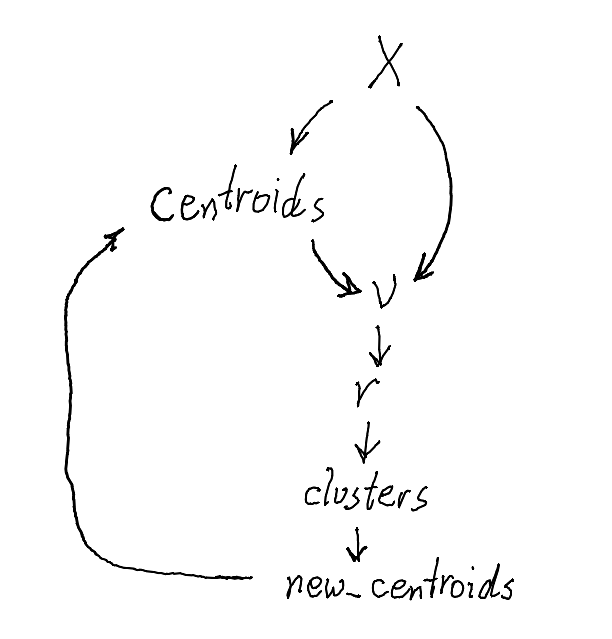
\includegraphics[width=3.7cm]{gfx/ex-dataflow.png}
};
\end{tikzpicture}
\caption{\label{lst:code-kmeans}
K-Means clustering with $k$ clusters.}
\end{figure}

\subsection{Running Example: K-Means Clustering}
\label{sec:running-example}

We illustrate our checkpointing approach using the classical \emph{K-Means clustering} algorithm~\cite{macqueen1967multivariate}. This widely used iterative method, partitions a dataset into $k$ clusters by repeatedly reassigning points to the nearest centroid and updating centroids as the mean of their assigned points.

Each iteration proceeds as follows:
\begin{enumerate}
    \item \textbf{Cluster assignment:} Each data point is assigned to its nearest centroid.
    \item \textbf{Centroid update:} New centroids are computed as the mean of each cluster.
    \item \textbf{Convergence check:} If centroids have not significantly changed, the algorithm halts.
\end{enumerate}

This style of computation is a natural fit for checkpointing: each iteration overwrites the previous cluster assignments and recomputes temporary data structures from scratch. Only the \texttt{centroids} array must persist across iterations. However, conventional checkpointing tools like CRIU or VM-based snapshots indiscriminately capture the full resident memory---including all temporary arrays and internal buffers---leading to high storage and I/O overhead.

Our system avoids this inefficiency by identifying the \emph{minimal} state necessary to resume execution after a crash. It does so through a static analysis pipeline that combines:
\begin{itemize}
    \item \textbf{Liveness analysis} to determine which variables are needed for future execution.
    \item \textbf{Points-to analysis} to track object references and heap structure.
    \item \textbf{Dirty analysis} to identify memory locations that were actually modified.
\end{itemize}
Applied to K-Means, the analysis concludes that only the centroid array is both live and dirty at the loop head. All other objects---including the \texttt{clusters} data structure, distance computations, and scratch space---are either recomputed or dead.

\begin{figure}[t]
\centering
\begin{lstlisting}[language=python]
# initialization unchanged
with Loader(__file__, locals()) as transaction:
    if transaction:
        [centroids] = transaction.move()
    for i in transaction.iterate(range(iters)):
        # Loop body unchanged
        transaction.commit(centroids)
# finalization unchanged
\end{lstlisting}
\caption{Automatic checkpoint injection at the loop header.}
\label{fig:checkpoint-injection}
\end{figure}

As shown in \autoref{fig:checkpoint-injection}, our instrumentation wraps the loop with a lightweight transactional API. This enables recovery after a crash by restoring execution to the loop head with the correct value of \texttt{i} and \texttt{centroids}, without persisting irrelevant data. It is technically possible to make the instrumentation less syntactically intrusive, but the intention is to make it clear to the developer what the instrumentation does.

\paragraph{Language Features and Implementation Twists}

Although K-Means is conceptually simple, its Python implementation highlights several challenges for static analysis in a dynamic language. In particular:
\begin{itemize}
    \item \textbf{Generic data structures.} The variable \texttt{clusters} is a list of lists of integers. In order to enable type-checking and proper tracking of its structure, we require the use of explicit type constructors such as \texttt{list[int]()}. This ensures that our analysis can infer a meaningful and consistent type.
    \item \textbf{Side effects.} Function calls such as \texttt{xs.append(y)} mutate nested list. Our dirty analysis correctly tracks such effects to determine whether the object needs to be persisted. However, in this case, \texttt{clusters} is reconstructed every iteration and does not need to be saved.
    \item \textbf{Effect annotations.} For functions like \texttt{np.array} and \texttt{np.linalg.norm}, we rely on an internal library of effect annotations that describe whether a function allocates a new object, updates its arguments, or returns an alias. For example, \texttt{np.array} is treated as a constructor (``new''), while \texttt{np.mean} is considered pure. These annotations are essential for tracking heap mutations and avoiding conservative over-approximation.
    \item \textbf{Control-flow simplification.} Because Python bytecode is complex, we translate it to a simplified intermediate representation for verification and analysis.
\end{itemize}

Despite the simplicity of the target algorithm, precise analysis demands careful handling of Python's typing and memory model. Our implementation supports this through a combination of expressiveness in the type domain and selective annotation of external APIs. The result is an end-to-end system that enables lightweight, high-frequency checkpointing with no manual specification of which variables to save.
